
\centerline{\textbf{ \LARGE Paging}}


% ----------------------------------------------------------------------------


\begin{enumerate}

  \begin{figure}[h]
      \centering   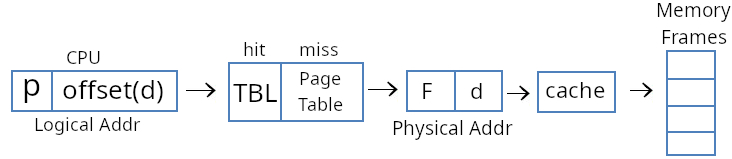
\includegraphics[scale=2.5]{./images/paging_01.jpeg}
  \end{figure}
  \item Paging \\
  \begin{myTableStyle}
    \begin{tabular}{ |m{3.5cm}|m{10cm}| } \hline
        Frame           &     Physical Address Space divided into frames                  \\ \hline
        Page            &     Logical   Address Space divided into pages.                 \\
                        &     Page size defined by hardware                               \\ \hline
        Page Table      &     maping of page no to frame no                               \\ \hline
        Word            &     Page Size = Frame Size =  \(2^k\) words                     \\ \hline
        offset(k-bits)  &     index of the word in a page/frame  \\ \hline
        Logical address &     page no(p)  +  offset(d)                                    \\ \hline
        Physical address&     frame no(f) +  offset(d)                                    \\ \hline
        Page Table Size &     \(2^p\) x size of one entry                                       \\
                        &     \(2^p\) = No of entries in page table = total pages                \\ \hline
        Translation \mbox{Lookaside} Buffer(TLB) & Acts as cache for page table                    \\ \hline
        Page Table Base \mbox{ Register} &                                                        \\ \hline
    \end{tabular}
  \end{myTableStyle}
  \vspace{0.08in}

  \item Each process has a page table.
  \item PT can not be in registers because registers are small in size.
  \item PT are kept in memory. Two main memory references are required to access a word in memory.
  \item Page table entry (PTE) \\
  \begin{myTableStyle}
    \begin{tabular}{ |m{2cm}|m{2cm}|m{2cm}|m{2cm}|m{3cm}| } \hline
        Page no &  Frame no & Valid bit & Dirty bit & Protection bit  \\ \hline
    \end{tabular}
  \end{myTableStyle}
  \vspace{0.08in}


  \item TLB : https://www.geeksforgeeks.org/translation-lookaside-buffer-tlb-in-paging/
    \begin{enumerate}
      \item Is a high-speed cache that stores a part of page table(PT).
      \item TLB miss : TLB is updated with new PTE.
      \item TLB entry replacement policies : FIFO, LRU or MFU etc
      \item TLB first checks. If the page is not in memory a page fault is issued then the TLB is updated to include the new page entry.
    \end{enumerate}
    \vspace{0.08in}

    \item Page sharing : multiple processes share the same  frame. Each PT will have an PTE for that frame.
    \vspace{0.08in}

    \item Single level page table \\

    \begin{myTableStyle}
    \begin{tabular}{ |m{1.5cm}|m{1cm}| } \hline
        Page no  &  offset  \\ \hline
        n-a   &   a         \\ \hline
    \end{tabular}
  \end{myTableStyle}
  \vspace{0.08in}

  \begin{myTableStyle}
    \begin{tabular}{ |m{4cm}|m{2cm}|m{5cm}| } \hline
        Page Size               &   \(2^a\)         & offset bits = a        \\ \hline
        Page Table Entry Size   &   \(2^e\)         &                         \\ \hline
        Physical Address Space  &   \(2^{f+a}\)     & f + a                 \\ \hline
        Logical Address Space   &   \(2^n\)         & (n-a) + a                 \\ \hline
        No of pages             &   \(2^{n-a}\)     &                         \\ \hline
        Page Table size         &   \(2^{n-a+e}\)   & need 1 page             \\ \hline
    \end{tabular}
  \end{myTableStyle}
  \vspace{0.08in}

  \item Two level page table \\

    \begin{myTableStyle}
    \begin{tabular}{ |m{2.5cm}|m{2.5cm}|m{1cm}| } \hline
        offset-1 & offset-2  &  offset  \\ \hline
        n-a-b   &   b  &  a         \\ \hline
    \end{tabular}
  \end{myTableStyle}
  \vspace{0.08in}

  \begin{myTableStyle}
    \begin{tabular}{ |m{4cm}|m{2cm}|m{5cm}| } \hline
        Page Size               &   \(2^a\)         & offset bits = a         \\ \hline
        Page Table Entry Size   &   \(2^e\)         &                         \\ \hline
        Physical Address Space  &   \(2^{f+a}\)     & f + a                   \\ \hline
        Logical Address Space   &   \(2^n\)         & n                       \\ \hline
        PTE in one page         &   \(2^{a-e}\)     & equals \(2^b\) (b=a-e)  \\ \hline
    \end{tabular}
  \end{myTableStyle}
  \vspace{0.08in}

  \begin{myTableStyle}
    \begin{tabular}{ |m{4cm}|m{3cm}|m{3cm}|m{3cm}| } \hline
                            &   Process             &   Page Table(L1)          &   Page Table(L2)        \\ \hline
        No of pages         &   \(2^{n-a}\)         &   \(2^{n-2a+e}\)          &   \(2^{n-3a+2e}\)       \\ \hline
        Page Table size     &   \(2^{n-a+e}\) (L1)  &   \(2^{n-2a+2e}\) (L2)    &   NA                    \\ \hline
    \end{tabular}
  \end{myTableStyle}
  \vspace{0.08in}

  \begin{minipage}{\linewidth}
  \item Three level page table \\

    \begin{myTableStyle}
    \begin{tabular}{ |m{2.5cm}|m{2.5cm}|m{2.5cm}|m{1cm}| } \hline
        offset-1 & offset-2 & offset-3  &  offset  \\ \hline
        n-a-b-c   &  c   &   b  &  a         \\ \hline
    \end{tabular}
  \end{myTableStyle}
  \vspace{0.08in}

  \begin{myTableStyle}
    \begin{tabular}{ |m{4cm}|m{2cm}|m{5cm}| } \hline
        Page Size               &   \(2^a\)         & offset bits = a         \\ \hline
        Page Table Entry Size   &   \(2^e\)         &                         \\ \hline
        Physical Address Space  &   \(2^{f+a}\)     & f + a                   \\ \hline
        Logical Address Space   &   \(2^n\)         & n                       \\ \hline
        PTE in one page         &   \(2^{a-e}\)     & equals \(2^b\) (b=c=a-e)\\ \hline
    \end{tabular}
  \end{myTableStyle}
  \vspace{0.08in}

  \begin{myTableStyle}
    \begin{tabular}{ |m{2.5cm}|m{2.5cm}|m{2.5cm}|m{2.5cm}|m{2.5cm}| } \hline
                            &   Process             &   Page Table(L1)          &   Page Table(L2)      &   Page Table(L3)        \\ \hline
        No of pages         &   \(2^{n-a}\)         &   \(2^{n-2a+e}\)          &   \(2^{n-3a+2e}\)     &   \(2^{n-4a+3e}\)       \\ \hline
        Page Table size     &   \(2^{n-a+e}\) (L1)  &   \(2^{n-2a+2e}\) (L2)    &   \(2^{n-3a+3e}\)(L3) &   NA                    \\ \hline
    \end{tabular}
  \end{myTableStyle}
  \vspace{0.08in}
  \end{minipage}


      \begin{figure}[h]
          \centering   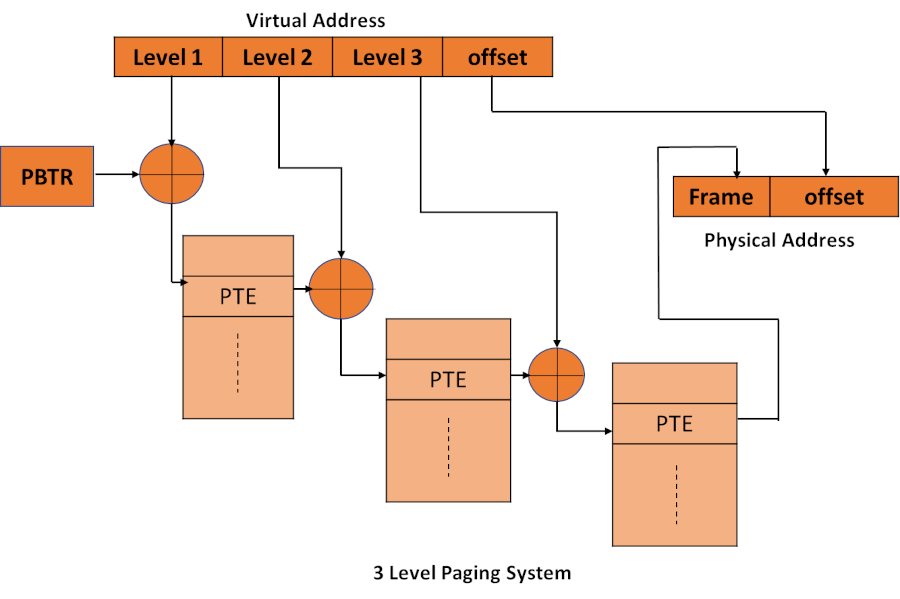
\includegraphics[scale=0.4]{./images/paging_03.jpeg}
      \end{figure}

      \item https://www.cs.utexas.edu/~lorenzo/corsi/cs372/06F/hw/3sol.html \\

    \begin{minipage}{\linewidth}
    \item Example of multi level page table.  \\

  \begin{myTableStyle}
    \begin{tabular}{ |m{4cm}|m{1cm}|m{5cm}| } \hline
        Page Size               &   \(2^{12}\) B  & offset bits = 12        \\ \hline
        Page Table Entry Size   &   \(2^{2}\)  B  &                         \\ \hline
        No of PTE in one page   &   \(2^{10}\) B  & offset bits for every level = 10        \\ \hline
        Physical Address Space  &   \(2^{44}\) B  & 32 + 12                 \\ \hline
        Logical Address Space   &   \(2^{32}\) B  & 10 + 10 + 12            \\ \hline
    \end{tabular}
  \end{myTableStyle}
  \vspace{0.08in}

    \begin{myTableStyle}
      \begin{tabular}{ |m{2cm}|m{2cm}|m{2cm}|m{2cm}|m{2cm}|m{2cm}| } \hline
          Process Size \(2^{32}\) B & size in pages & PTE         &  PT-size        &  PT-size              \\ \hline
          Process                   &  \(2^{20}\)   &  \(2^2\) B  &  \(2^{22}\) B   &  \(2^{10}\) page    \\ \hline
          L-2 PT                    &  \(2^{10}\)   &  \(2^2\) B  &  \(2^{12}\) B   &  1 page             \\ \hline
          L-1 PT                    &  1            &  NA         &  NA             &  1 page               \\ \hline
      \end{tabular}
    \end{myTableStyle}
    \vspace{0.08in}

    \end{minipage}


    \begin{minipage}{\linewidth}
    \item Example of multi level page table.  \\

  \begin{myTableStyle}
    \begin{tabular}{ |m{4cm}|m{1cm}|m{5cm}| } \hline
        Page Size               &   \(2^{20}\) B  & offset bits = 20        \\ \hline
        Page Table Entry Size   &   \(2^{2}\)  B  &                         \\ \hline
        No of PTE in one page   &   \(2^{18}\) B  & offset bits for every level = 18        \\ \hline
        Physical Address Space  &                 &                          \\ \hline
        Logical Address Space   &   \(2^{64}\) B  & 8 + 18 + 18 + 20            \\ \hline
    \end{tabular}
  \end{myTableStyle}
  \vspace{0.08in}

    \begin{myTableStyle}
      \begin{tabular}{ |m{2cm}|m{2cm}|m{2cm}|m{2cm}|m{2cm}|m{2cm}| } \hline
          Process Size \(2^{64}\) B & size in pages & PTE         &  PT-size        &  PT-size              \\ \hline
          Process                   &  \(2^{44}\)   &  \(2^2\) B  &  \(2^{46}\) B   &  \(2^{26}\) pages     \\ \hline
          L-3 PT                    &  \(2^{26}\)   &  \(2^2\) B  &  \(2^{28}\) B   &  \(2^{8}\)  pages     \\ \hline
          L-2 PT                    &  \(2^{8}\)    &  \(2^2\) B  &  \(2^{10}\) B   &   1 page               \\ \hline
          L-1 PT                    &  1            &  NA         &  NA             &   1 page              \\ \hline
      \end{tabular}
    \end{myTableStyle}
    \vspace{0.08in}
    \end{minipage}

    \begin{minipage}{\linewidth}
    \item Example of level-3 page table.\\
    \begin{myTableStyle}
      \begin{tabular}{ |m{2cm}|m{2cm}|m{2cm}|m{2cm}| } \hline
                  10-bit &  8-bit & 6-bit & 8-bit \\ \hline
      \end{tabular}
    \end{myTableStyle}
    \vspace{0.08in}


    \begin{myTableStyle}
      \begin{tabular}{ |m{2cm}|m{2cm}|m{2cm}|m{2cm}|m{2cm}| } \hline
          Process Size \(2^{18}\) B  & offset bits & Maximum PTEs/Bytes in single page & total PTEs/Bytes  & total pages\\ \hline
          Process   &   8   &  \(2^8\) B      &   \(2^{18}\) B&   \(2^{10}\)    \\ \hline
          Level-3   &   6   &  \(2^6\)        &   \(2^{10}\)  &   \(2^{4}\)     \\ \hline
          Level-2   &   8   &  \(2^8\)        &   \(2^{4}\)   &   1             \\ \hline
          Level-1   &   10  &  \(2^{10}\)     &   1           &   1             \\ \hline
      \end{tabular}
    \end{myTableStyle}

    PTE size =  2B \\
    total size needed to store page table = (\(2^{10}\) x 2)  + (\(2^{8}\) x 2)  + (\(2^{10}\) x 2)
    \vspace{0.08in}
  \end{minipage}





\end{enumerate}

% ----------------------------------------------------------------------------

% ----------------------------------------------------------------------------

% ----------------------------------------------------------------------------

% ----------------------------------------------------------------------------

% ----------------------------------------------------------------------------

% ----------------------------------------------------------------------------

% ----------------------------------------------------------------------------

% ----------------------------------------------------------------------------
